\section{Kapacitetsudnyttelse} \label{kap}
% Skriv ift kapacitet (ift sengepladser, persona - hvilken betydning har hhv. 95 \% kapacitet mod 105 \%)
Kapacitetudnyttelse betegner forholdet mellem aktivitet og kapacitet. Aktivitet omhandler patient og kontakt, herunder består kontakt af forundersøgelse, behandling og kontrol. Kapacitet omfatter antallet af personale, udstyr og rum, hvor personalet består af læger, sygeplejersker og sekretærer. Udstyret beskriver antallet af maskiner på en afdeling og antallet af rum beskriver opbevarelsen af udstyret. Den samlede kapacitetsudnyttelse er defineret ud fra, at der produceres mest muligt for de investerede ressourcer.\cite{Company2013} 

\begin{figure}[H]
	\flushleft 
	\centering
	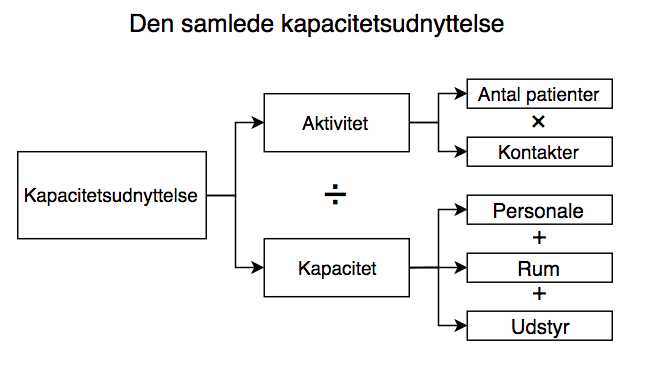
\includegraphics[scale=.5]{figures/Kapacitetsudnyttelse.png}
	\flushleft
	\caption{\textit{Den samlede kapacitetsudnyttelse, som er definineret ved forholdet mellem aktivitet og kapacitet. Aktivitet omfatter antallet af patienter samt kontakter og kapacitet omfatter personale, rum og udstyr.}\cite{Company2013}}
	\label{kapacitet}
\end{figure}

\noindent
Ud fra \figref{kapacitet} fremgår det, at kapacitetsudnyttelse er forholdet mellem aktivitet og kapacitet. Dertil ses aktivitet som antal patienter multipliceret med kontakter. Kapaciteten udgør personale, rum og udstyr lagt sammen. Antallet af patienter, der repræsenterer en del af aktivitet beskriver ligeledes belægning på hospitalets afdelinger.\cite{Company2013} 

Belægning er defineret ud fra antallet af patienter, der er normeret til på en afdeling\cite{Heidmann2014}. Når en $100~\%$ belægning opnås, svarer dette til, at de disponible sengepladser på en afdeling er taget i brug. Ved en belægning på over $100~\%$ betyder det, at der er flere patienter end afdelingen er normeret til, hvilket vil sige, at afdelingen yder mere end der er kapacitet til. Ud fra \figref{kapacitet} vil dette betyde, at der ikke er ligevægt mellem aktivitet og kapacitet, hvilket i dette tilfælde vil forårsage kapacitetsmangel på afdelingen. Det kan derfor være nødvendigt, at personalet skal varetage flere patienter samt arbejdsopgaver. Herudover kan det være nødvendigt at tilkalde ekstra personale for at opnå en balance i kapacitetsudnyttelsen.
Hvis der derimod er en belægning på under $100~\%$ er der omvendt færre patienter end afdelingen er normeret til. Dette betyder, at der er flere sengepladser end patienter, hvilket ligeledes fører til en ubalance i kapacitetsudnyttelsen. I denne situation er der mere personale end nødvendigt, hvilket betyder, at der ikke er fuld udnyttelse af personalets arbejdskraft.\cite{Pauly1986} 

Det anses herved vigtigt, at der er balance mellem aktivitet og kapacitet, således de investerede ressourcer udnyttes optimalt. Det ønskes derfor at opnå en kapacitetsudnyttelse på $100~\%$. Ud fra dette vil der fremover undersøges betydningen af kapacitetsudnyttelse på ortopædkirurgisk afdeling på Aalborg Universitetshospital. 

\subsection{Ortopædkirurgisk afdeling} \label{kap_OA}
Ortopædkirurgisk afdeling på Aalborg Universitetshospital behandler skade på knogler, muskler, sener eller led. Dette gøres indenfor 10 fagområder: Børneortopædkirurgi, knogle- og rekonstruktion, fod- og ankelkirurgi, knæ- og hoftekirurgi, håndkirurgi, ryg- og bækkenkirurgi, knæ- og idrætsskader, tumor- og sarkomkirurgi, amputationer samt sår og traumatologi.\cite{Aalborg2016} Fordelingen af operationer foretaget på ortopædkirurgi afdeling i perioden 1. august til 31. oktober fremgår af \figref{operationstype}. 

\begin{figure}[H]
	\flushleft 
	\centering
	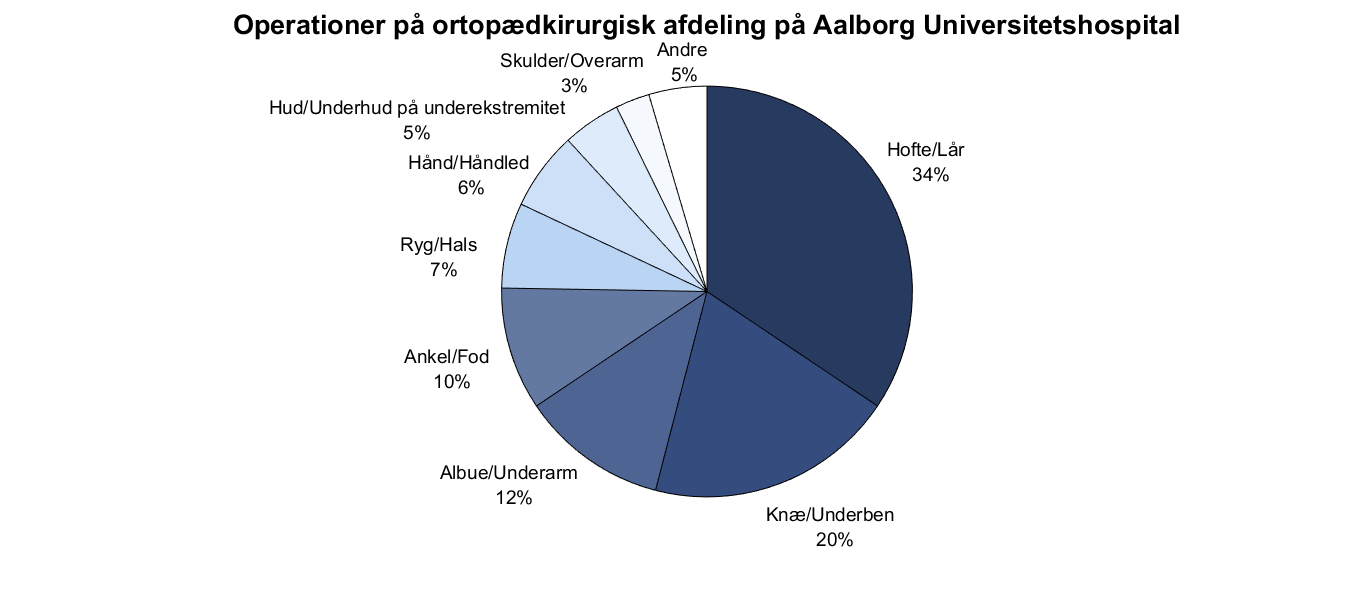
\includegraphics[scale=0.55]{figures/operationsdiagram.png}
	\flushleft
	\caption{\textit{Fordelingen af operationer foretaget på ortopædkirurgisk afdeling på Aalborg Universitetshospital i perioden 1. august til 31. oktober år 2014. Andre består af: Ydre øre, mindre kirurgi på bevægeapparatet, rygmarv og nervebrud, perifer nerver, hud og underhud på truncus, hud og underhud på overekstremiteter.}}
	\label{operationstype}
\end{figure}

\noindent
Fordelingen af operationer foretaget på ortopædkirurgisk afdeling på Aalborg Universitetshospital fremgår af \figref{operationstype}. Størstedelen af operationer er hofte/lår og knæ/underben, hvilket samlet udgør 54 \% af alle operationer.

\subsubsection{Budget på ortopædkirurgisk afdeling}
Kapacitetsudnyttelse afhænger af det budget som hver afdeling har til rådighed. Dette budget udregner Sundhedsstyrrelsen ud fra diagnoserelaterede grupper (DRG). DRG anvendes til at analysere omkostninger og aktivitet på et hospital.\cite{DRG2016} Ortopædkirurgisk afdeling har et budget på $700.872.744$ kr, som svarer til 17,2 \% af det samlede budget for alle afdelinger på Aalborg Universitetshospital. Det samlede DRG for afdelingerne på Aalborg Universitetshospital er illusteret af \figref{DRG_budget}.\cite{Rasmussen2016}
Størstedelen af budgettet anvendes til personale- og patientudgifter, som svarer til hhv. 60 \% og 32 \%. Det resterende budget anvendes til bygninger, it, apparatur, inventar samt drift og service\cite{Noegletal2016}. 


\begin{figure}[H]
	%\flushleft 
	\centering
	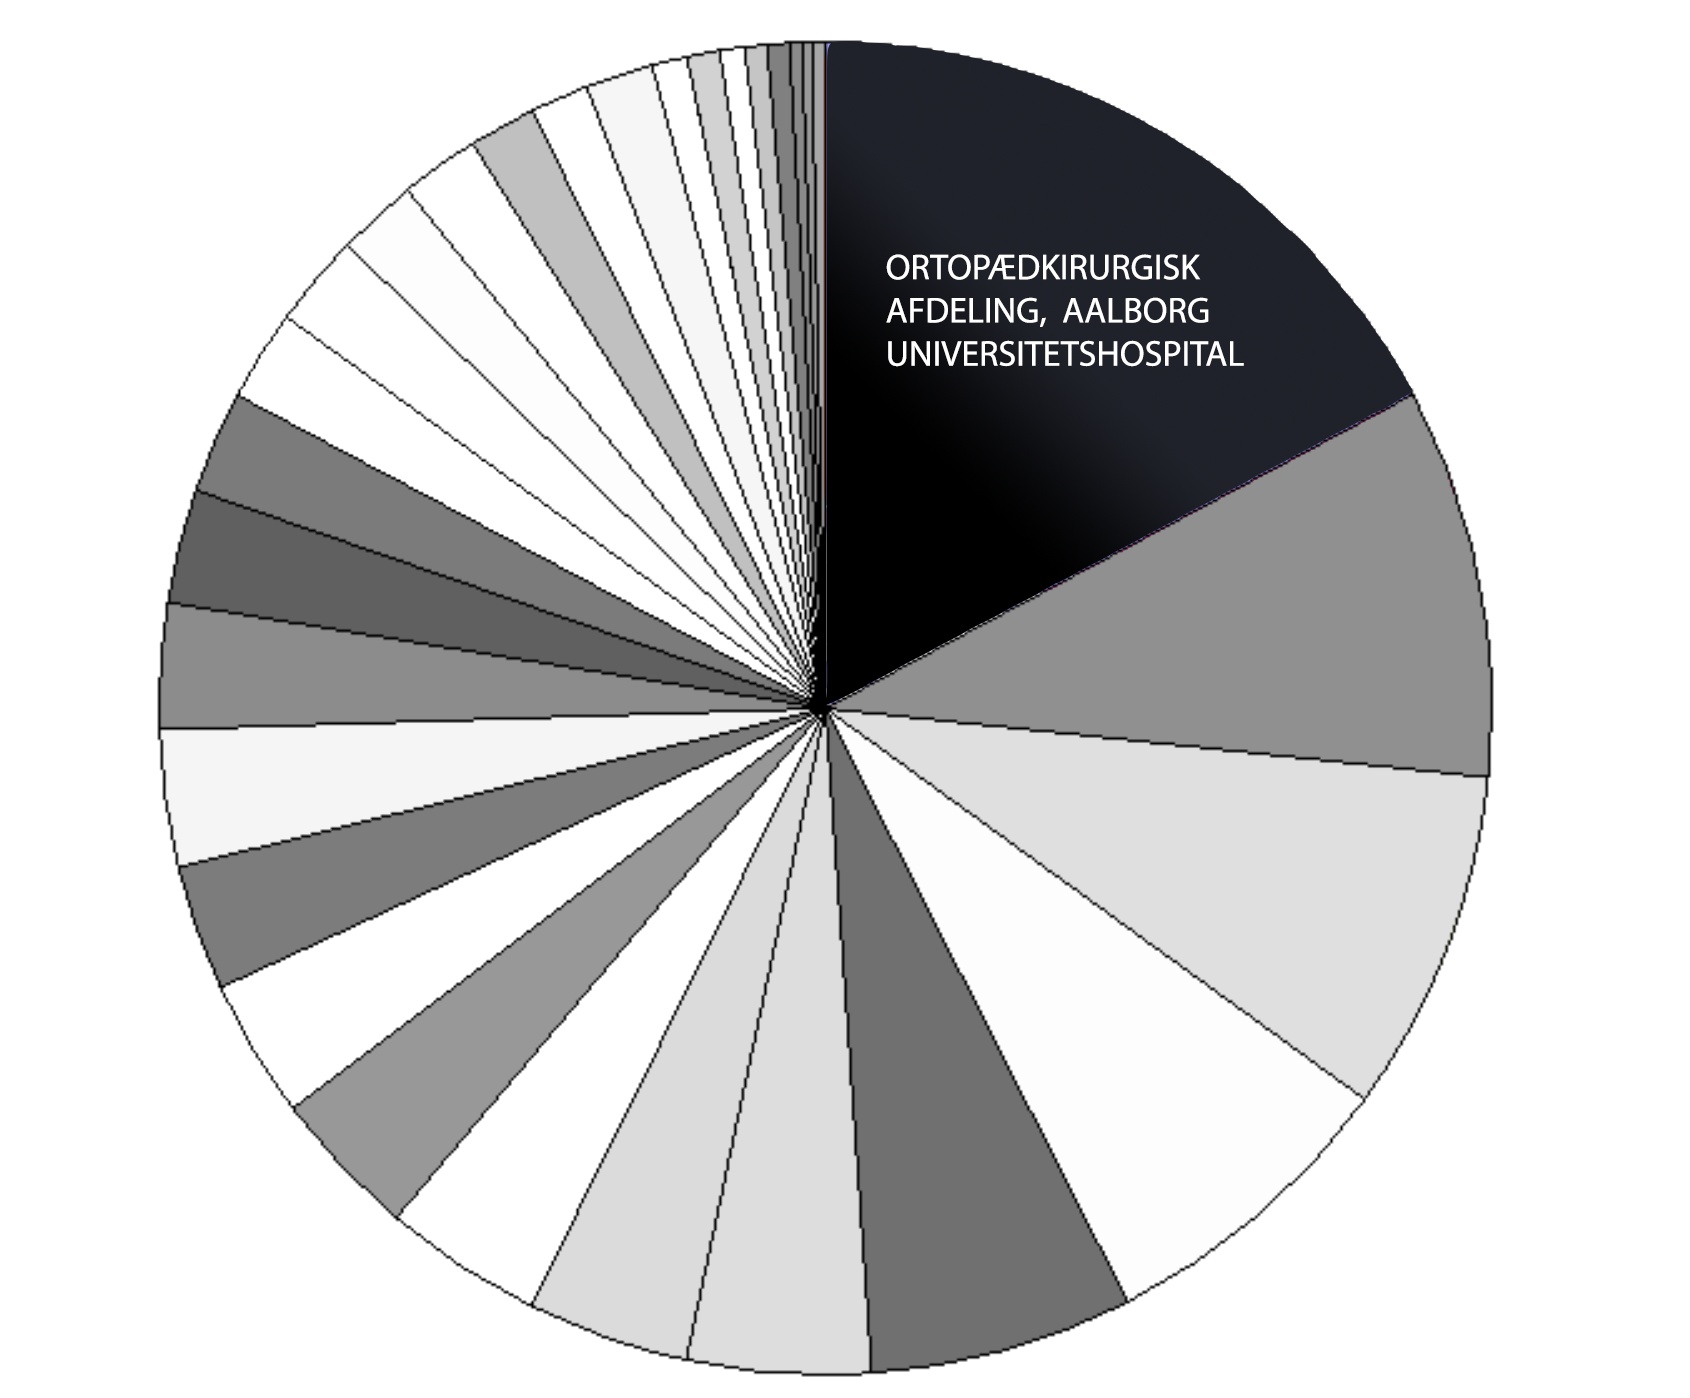
\includegraphics[scale=0.45]{figures/Ortopaeddiagram.png}
	%\flushleft
	\caption{\textit{Fordeling af DRG for samtlige afdelinger på Aalborg Universitetshospital. Det fremgår, at ortopædkirurigisk afdeling har en større andel end de resterende afdelinger.}\cite{Rasmussen2016}}
	\label{DRG_budget}
\end{figure}


\subsubsection{Personalearbejde} 
På ortopædkirurgisk afdeling på Aalborg Universitetshospital arbejder personalet i gennemsnit 37 timer om ugen\cite{Danske2015}, hvorunder der både kan være nat- og dagvagter. Over en arbejdsdag er der indlagt tre vagtskifte, hvor det nye vagthold har et kvarter til at sætte sig ind i, hvilke opgaver samt patienter de skal varetage. Der er indlagt betalte pauser, hvilket betyder, at personalet skal være til rådighed under pausen. Personalet arbejder ofte i par, hvor de sammen varetager 2-8 patienter om dagen, mens de ofte varetager flere patienter på aftenvagter.\ref{bilagA} 


\subsubsection{Patientindlæggelse} 
Som beskrevet i afsnit \ref{kap} ønskes en $100~\%$ kapacitetsudnyttelse, dertil ønskes ligeledes en belægning på $100~\%$. 
For at opfylde dette skal der være ligevægt mellem antallet af sengepladser og patientindlæggelser. På ortopædkirurgisk afdeling er der $84$ til $120$ disponible og $125$ til $129$ normerede sengepladser over en $18$ måneders periode fra januar $2014$ til juni år $2015$. 

Ortopædkirurgisk afdeling modtager både elektive samt akutte patienter. Elektive patienter omfatter både indlagte og ambulante patienter. Ved pludselig forværret tilstand kan elektive patienter skifte status fra elektiv til akut. Akutte patienter defineres som personer, der er henvist til hospitalet efter en akut opstået tilstand. Sammenlignes der med de resterende afdelinger på Aalborg Universitetshospital, har ortopædkirurgisk afdeling flest elektive indlæggelser.\cite{RegionNord2016} En fordeling af de elektive og akutte patienter fremgår af \figref{elektivvsakut}.

\begin{figure}[H]
	\flushleft 
	\centering
	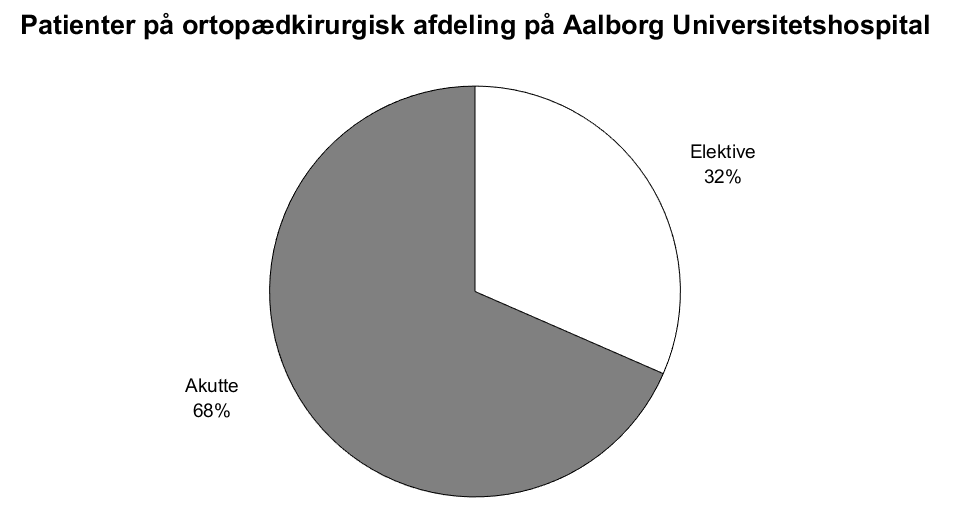
\includegraphics[scale=0.55]{figures/elektivvsakut.png}
	\flushleft
	\caption{\textit{Fordeling af elektive og akutte patienter på ortopædkirurgisk afdeling på Aalborg Universitetshospital målt over en tre måneders periode fra august til november år 2014.}}
	\label{elektivvsakut}
	\end{figure}

\noindent
Af \figref{elektivvsakut} illustreres det, at fordelingen mellem elektive og akutte patienter ikke er ligeligt fordelt på ortopædkirurgisk afdeling. Der ses over en tre måneders periode i år 2014, at de elektive patienter udgør $32~\%$ og de akutte udgør $68~\%$ af de samtlige patienter. \\

\noindent
\textbf{Indlæggelse- og udskrivelsestidspunkt} \\
På ortopædkirurgisk afdeling på Aalborg Universitetshospital foregår bookingen af elektive patienter med forbehold for akutte patienter. Dette betyder, at samtlige sengepladser ikke udnyttes fuldt ud. Operationstiden planlægges ofte ud fra patienternes eget ønske, der kan her være et ønske om en bestemt kirurg, tidsperiode eller blot den første ledige tid.\ref{bilagA} Indlæggelses- og udskrivelsestidspunktet for akutte og elektive i perioden august til oktober år $2014$ fremgår af \figref{indlaegudskriv}. 


\begin{figure}[H]
	%\flushleft 
	\centering
	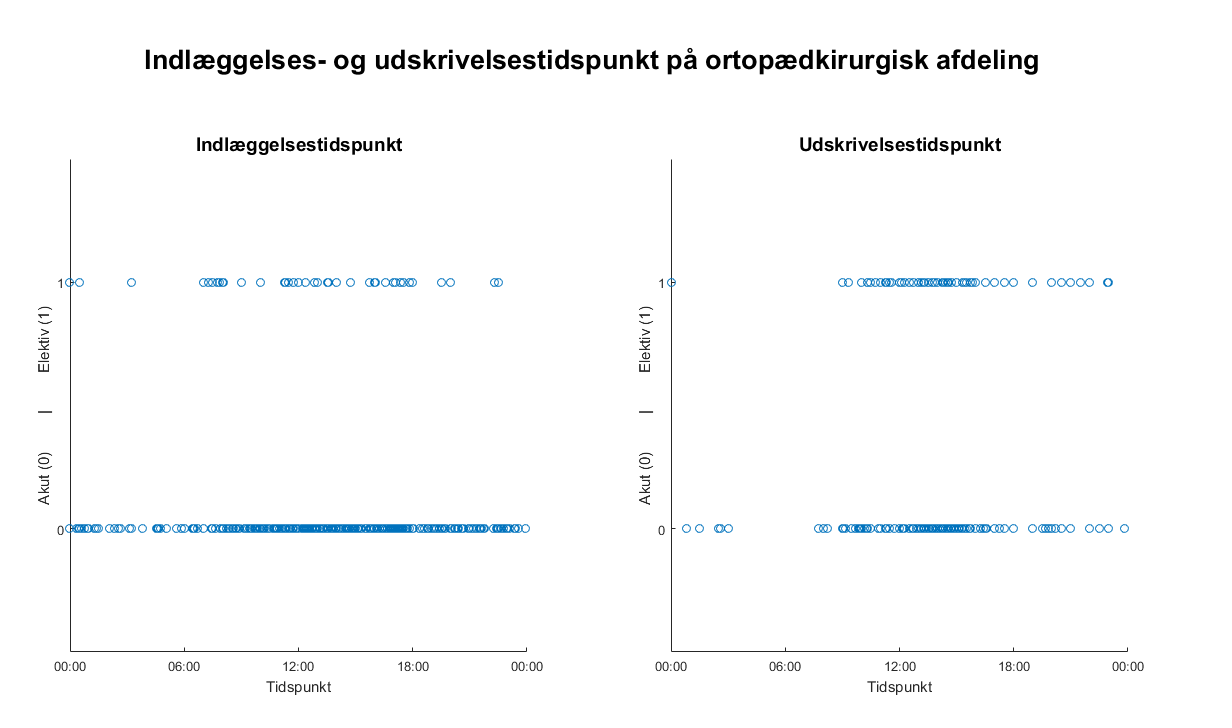
\includegraphics[scale=0.5]{figures/indlaegudskriv.png}
	%\flushleft
	\caption{\textit{Indlæggelse- og udskrivelsestidspunkt for akutte og elektive patienter over en 3 måneders periode fra august til oktober 2014.}}
	\label{indlaegudskriv}
	\end{figure}
	
\noindent
På \figref{indlaegudskriv} fremgår indlæggelses- og udskrivelsestidspunkter for akutte og elektive patienter. Indlæggelsestidspunktet for elektive ses typisk mellem kl. 7 og 18, hvorimod de akutte indlæggelses i løbet af hele døgnet. Udskrivelsestidspunktet for elektive ses typisk melem kl. 9 og 18, mens akutte typisk udskrives mellem kl. 8 og 18. 